\section{Winch Hydraulics}

Modeling of a hydraulic system allows limitations of the winch as an actuator and the load it puts on the engine to be realized. The system components contain a pressure-compensated, variable displacement piston pump, a fixed displacement piston motor, a four-way two-position valve, a pressure relief valve, and a braking valve \cite{MathWorks2015bb,MathWorks2015a,MathWorks2015PressureReliefValve}. The schematic for the proposed system is shown in Fig. 19. The two-position valve allows for two modes of operation: pulling in the towed load and braking. In Fig. \ref{fig:Winch_Hydraulics_Diagram}, the position selected is for braking (II) and connects all four ways. This eliminates any pressure differential between $P_H$ and $P_O$ and activates the braking valve denoted as B2. The equations describing the pressure-rise rate within the section of hose $P_O$ in this mode of operation are given by \cite{manring1998modeling}
\begin{equation}\label{eq:VP2_eq1}
    P_H = 0
\end{equation}
\begin{equation}\label{eq:VP2_eq2}
    \dot P_O = \frac{\beta}{V_O}Q_O
\end{equation}
\begin{equation}\label{eq:VP2_eq3}
    Q_O = D_M\omega_M - q_{B2}
\end{equation}
\begin{equation}\label{eq:VP2_eq4}
q_{B2} = \left\{
        \begin{array}{ll}
            q_{leak} & \quad P_O \leq P_{set} \\
            q_{leak} + k_{B2}(P_O - P_{set}) & \quad P_{set} < P_O < P_{Max} \\
            q_{B2,Max} & \quad P_O \geq P_{Max}
        \end{array}
    \right.
\end{equation}
\begin{equation}\label{eq:VP2_eq5}
    k_{B2} = (q_{B2,Max}-q_{leak})/P_{Max}
\end{equation}
\begin{equation}
    D_P = 0
\end{equation}
\begin{equation}
    \tau_{P} = 0
\end{equation}
\begin{equation}
    \tau_W = D_M P_O g_M
\end{equation}
\begin{equation}
    \omega_P = \omega_E g_P
\end{equation}
\begin{equation}\label{eq:VP2_end}
    \omega_M = \dot\psi g_M
\end{equation}
\begin{figure}[tb]
    \centering
    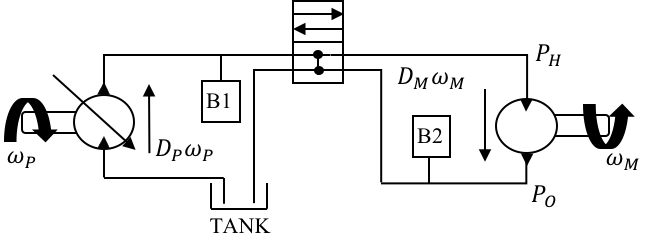
\includegraphics[width = 4in, keepaspectratio]{WINCH_HYDRAULICS_DIAGRAM_VP2}
    \caption{Hydraulics circuit schematic for the winch implement. The element on the far left denotes a pressure compensated, variable displacement hydraulic pump that connects to the engine through a constant gear ratio $g_P$. The element on the far right is a fixed displacement hydraulic motor that is connected to the winch element through a constant gear ratio $g_M$. The element in the middle is 4 way, 2 position hydraulic valve. The current valve selection is for operation in brake mode where all four ways are connected and is denoted as position II. Position I is used for reeling in the payload and allows the variable displacement piston pump to the engine to create a pressure differential for winch torque.}
    \label{fig:Winch_Hydraulics_Diagram}
\end{figure}
The model used for the braking valve is the same as for a pressure relief valve to regulate hydraulic pressure. The valve set relief pressure, $P_{set}$ is an input that modulates how much braking torque to use for the hydraulic motor in the winch.

The other position of the four-way two-position valve (I) isolates the sections of hose, $P_H$ and $P_O$ to create a pressure differential driven by the piston pump connected to the engine. The equations in this mode of operation are given by 
\begin{equation}\label{eq:VP1_eq1}
    \dot P_H = \frac{\beta}{V_H}Q_H
\end{equation}
\begin{equation}\label{eq:VP1_eq2}
    P_O = 0
\end{equation}
\begin{equation}\label{eq:VP1_eq3}
    Q_H = D_P\omega_P + D_M\omega_M - q_{B1}
\end{equation}
\begin{equation}\label{eq:VP1_eq4}
q_{B1} = \left\{
        \begin{array}{ll}
            q_{leak} & \quad P_H \leq P_R \\
            q_{leak} + k_{B1}(P_H - P_R) & \quad P_R < P_H < P_{Max} \\
            q_{B1,Max} & \quad P_H \geq P_{Max}
        \end{array}
    \right.
\end{equation}
\begin{equation}\label{eq:VP1_eq5}
    k_{B1} = (q_{B1,Max}-q_{leak})/P_{Max}
\end{equation}
\begin{equation}\label{eq:D_PII}
D_P = \left\{
        \begin{array}{ll}
            D_{P,Max} & \quad P_H \leq P_{set} \\
            D_{P,Max} - k_P(P_H - P_{set}) & \quad P_{set} < P_H < P_{Max} \\
            0 & \quad P_H \geq P_{Max}
        \end{array}
    \right.
\end{equation}
\begin{equation}\label{eq:VP1_eq7}
    k_P = D_{P,Max}/(P_{Max} - P_{set})
\end{equation}
\begin{equation}\label{eq:VP1_eq8}
    \tau_{P} = D_P P_H g_P
\end{equation}
\begin{equation}\label{eq:VP1_eq9}
    \tau_W = D_M P_H g_M
\end{equation}
\begin{equation}\label{eq:VP1_eq10}
    \omega_P = \omega_E g_P
\end{equation}
\begin{equation}\label{eq:VP1_eq11}
    \omega_M = \dot\psi g_M
\end{equation}
This mode of operation for the hydraulics allows the winch to pull in the towed load. The value $P_{set}$ in \ref{eq:D_PII} is an input to the variable displacement, pressure-compensated pump to maintain a pressure set point for $P_H$. This modulates the amount of torque the motor uses to pull in the towed load.